\chapter{State of the art}
Die Verkehrsstrategie des Senats sieht vor, dass das Radfahren bis zum Jahr 2025 20 Prozent des Gesamtverkehrs ausmachen soll. \cite{Mopo}
"Wir brauchen eine intelligente Konstruktion, die alle Verkehrsarten verbindet", sagte Stadtentwicklungssenator Michael Müller (SPD).\\
Sowohl statisch an Radwegen, als auch für den Einsatz in Kraftfahrzeugen gibt es bereits Projekte zu Ampelassistenten in Bordcomputern, Navigationssystemen, oder aber auch als App die rote Ampeln erkennen und die optimale Fahrtgeschwindigkeit für die Grüne Welle ermitteln. Auch Erweiterungen für's Rad direkt werden vielfältiger --- vom einfachen Navigationssystem bis hin zu intelligenten Aufsätzen, die an das Smartphone gekoppelt sind.
\gls{C2X}- Kommunikation oder/und \gls{GLOSA} definieren?
% ### Auto ###
\section{Ampelinformationssysteme}
Unter dem Prinzip "'Grüne Welle"' wird die Abstimmung der Ampelschaltzustände, sodass ein Fahrzeug in einer bestimmten Geschwindigkeit mehrere Ampeln passieren kann ohne anzuhalten, verstanden. Der folgende Abschnitt soll die existierenden Lösungen und Ansätze für Ampelinformationssysteme darstellen.
\subsection{Grüne Welle auf Radwegen}
In Kopenhagen unterstützen grüne \gls{LED}s auf Radwegen die Radfahrer indem sie wenn diese mit einem Tempo von 20 km/h fahren, sie begleiten und so signalisieren, dass sie sich auf der Grünen Welle befinden. 
\begin{figure}[H]  
    \centering  
    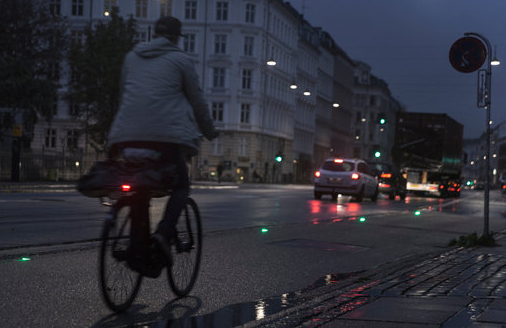
\includegraphics[width=0.7\textwidth]{copenhagen} \label{fig:copenhagen}
    \caption[Grüne Welle durch \gls{LED}s]{\gls{LED}s signalisieren die Grüne Welle bei 20 km/h  Quelle: \cite{NYT}}
\end{figure}
Zusätzlich erkennen Sensoren im Radweg Fahrradgruppen und veranlassen dann die Ampel zu einer längeren Grünphase. In einem anderen Stadtteil sind Leuchttafeln, die die verbleibende Zeit der Ampelphase anzeigen, am Radwegrand installiert\footnote{\cite{KopIng}}.\\
Mit Kopenhagen als Vorbild hat Berlin mit vier Ampeln in Schöneberg eine Grüne Welle für RadfahrerInnen umgesetzt und plant bereits die zweite\footnote{\cite{BZ}}. Auch hier möchte man die Benutzung des Rades attraktiver machen und den Fahrradverkehr beschleunigen.
\subsection{Projekt Wolfsburger Welle}
Die \gls{VW}-Forschung initiierte in den 80er Jahren mit dem Projekt "'Wolfsburger Welle"' die ersten Untersuchungen zur "'Grünen Welle"' Informationen im Fahrzeug; mit der Idee, beim Annähern an eine Ampel die optimale Geschwindigkeit im Fahrzeug zu geben.\footnote{\cite{Welle}} "Dazu sendet die Ampelanlage ihren aktuellen Phasenzustand und eine Prognose für den nächsten Zustandwechsel an alle Fahrzeuge, die sich annähern. Der Fahrzeugcomputer setzt dann die aktuelle Fahrzeuggeschwindigkeit mit dem Abstand zur Ampel und der aktuellen Ampelphase in Bezug. Daraus wird errechnet, ob das Fahrzeug im Moment mit der grünen Welle ’mitschwimmt’ oder ob die Geschwindigkeit außerhalb des optimalen Bereichs liegt" \cite{MenschMaschine}.
\subsection{Projekt Travolution}
Im Sommer 2008 wurde das Projekt \textsc{Travolution} (TRAffic \& eVOLUTION), von dem Amt für Verkehrsmanagement und Geoinformation der Stadt Ingolstadt, Audi AG\footnote{ Automobilhersteller, dem Volkswagen-Konzern zugehörig}, GEVAS Software\footnote{ Softwareunternehmen für Verkehrstechnik} und dem Lehrstuhl für Verkehrstechnik an der \gls{TUM} abgeschlossen. Es besteht aus den Teilprojekten \textsc{verkehrsadaptive Netzsteuerung mit Genetischen Algorithmen} und \textsc{Der informierte Fahrer}. Im Netzsteuerungsprojekt wurden 46 Lichtsignalanlagen in Ingolstadt mit der Netzsteuerungssoftware BALANCE ausgestattet, wodurch sie intelligent auf den Verkehr reagieren und die Schaltung an den Verkehr anpassen. 
\begin{figure}[H]  
    \centering  
    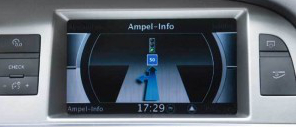
\includegraphics[width=0.7\textwidth]{audi-travolution}  \label{fig:travolution}
    \caption[Projekt Travolution]{\gls{C2I}-Kommunikation: Der Bordcomputer zeigt die optimale Geschwindigkeit an, sodass die nächste Kreuzung ohne Halt überquert werden kann. Quelle: {\url{http://www.audiusanews.com/imagegallery/adhoc/12647//12647,12649,12652,12648,12651,12650,/travolution-promotes-eco-friendly-driving}}}
\end{figure}
Ziel des zweiten Teilprojektes ist es, die Autofahrer über die Ampelphasen zu informieren. Die \gls{C2I}-Kommunikation mittels \gls{WLAN} und \gls{UMTS} umsetzend, senden mit Kommunikationsmodulen ausgestattete Ampeln die Grünphasen an den Bordcomputer der Autos, welcher widerum die Geschwindigkeit für ein reibungsloses Passieren errechnet\footnote{\cite{Travolution, AudiTravolution}}.\\ 
Fundierend auf \textsc{Travolution} wurden Folgeprojekte wie zum Beispiel das ebenfalls von Audi ins Leben gerufene "'Ampelinfo online"'. Über Mobilfunk ist in der \gls{C2X}-Anwendung das Auto mit dem zentralen Verkehrsrechner, welcher die Ampelanlagen steuert, vernetzt und visualisiert die entsprechenden Informationen im Bordcomputer. \footnote{\cite{Ampelinfo}}
%%% KOLIBRI %%%
\subsection{Projekt Kolibri}
In Bayern wurde im April 2011 das Pilot-Projekt \textsc{KOLIBRI} ("'Kooperative Lichtsignaloptimierung -- Bayrisches Pilotprojekt"') mit den Teststrecken der B13 bei München mit sieben und der St2145 in der Nähe von Regensburg mit acht ampelgeregelten Kreuzungen gestartet. Gemeinsam untersuchten TRANSFER GmbH\footnote{ ein Beratungs- und Softwareunternehmen für Transport und Verkehr}, die \gls{BMW} Group, der Lehrstuhl für Ergonomie an der \gls{TUM} und die Oberste Baubehörde im Bayerischen Innenministerium die Funktionen und Auswirkungen eines Ampelassistenten außerhalb von Ortschaften\footnote{\cite{kolibri}, \cite{kolibriTUM}}. "'Per Mobilfunk übermittelt das Fahrzeug Rohdaten wie Zeit und genaue Position. Der Computer in der Zentrale kann daraus Informationen über die Verkehrslage, die Geschwindigkeit oder die Zahl der Ampelstopps und die Wartezeiten ermitteln, die dann als Korrekturgrößen wieder in die Steuerung der Lichtsignalanlage einfließen können."'(\cite{kolibriTUM}) Zusätzlich wurden die Fahrer sowohl fahrzeugintegriert\footnote{ On-Board-Computer} als auch via Smartphone über die Schaltung der nächsten Ampel informiert und erhielten Empfehlungen über die aktuelle Progressionsgeschwindigkeit. 
\subsection{Projekt Testfeld Telematik}
Ende des Jahres 2013 wurde in Wien das Projekt \textsc{Testfeld Telematik} -- Feldversuch zur Stärkung österreichischen Know-Hows im Bereich umweltverträglicher Mobilität erfolgreich abgeschlossen. Per \gls{C2X-glo}-Kommunikation bringt das Projekt unter Kooperative Dienste wie Ampelinformationen direkt ins Auto. Über Navigationssysteme, integrierte Systeme, Nachrüst-Plattformen oder mobile Endgeräte erreicht die FahrerInnen die Information der optimalen Geschwindigkeit sowie die Dauer der jeweiligen Ampelphase. Um an die Informationen zu kommen wurden unter anderem Kameras und Sensoren, beispielsweise als Induktionsschleife in die Fahrbahn eingelassen\footnote{\cite{Siemens}}.
%Die Kommunikation zwischen den beteiligten Objekten verlief über ITS-GS, WAVE, CALM-IR und Mobilfunk.
\begin{figure}[H]
    \centering
    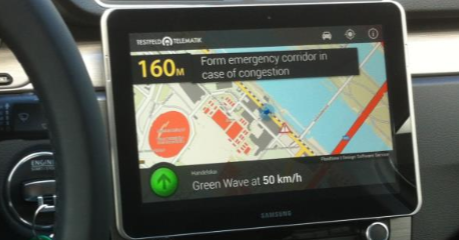
\includegraphics[width=0.7\textwidth]{telematik} \label{fig:telematik}
    \caption[Projekt Testfeld-Telematik Ampelinformation]{"'Grüne Welle bei 50 km/h"'  Quelle: \cite{Telematik}}
\end{figure}
Andere Autohersteller wie \gls{BMW}, Volvo und Volkswagen kooperieren als Forschungsprojekt "'Car 2 Car Communication Consortium"' mit \textsc{Testfeld Telematik}, ebenfalls mit dem Ziel die Sicherheit an Kreuzungen zu verbessern. Im Auto installierte Sensoren kommunizieren mit Kameras und Scanner in der Ampel. Allerdings funktioniert das System nur mit dem ambitionierten Ziel, wenn alle Autohersteller zusammenarbeiten und sich auf den gleichen Standard einigen.\footnote{\cite{Siemens}}
%TOYOTA 
\\ \textbf{WO SOLL DER TOYOTA ABSCHNITT HIN??? :} \\
Auch Toyota hat ein System entwickelt, welches eine spezielle Infrastruktur an Kreuzungen, die Installation von Infrarot-Sendern, die mit dem Toyota-Navigationssystem kommunizieren erfordert. An roter Ampel werden die Fahrer über die verbleibende Wartezeit informiert. Die ausgestatteten Navigationssysteme wurden bis jetzt jedoch ausschließlich in Japan getestet.\footnote{\cite{Toyota}}
%
%%% Apps %%% 
%
\section{Ampelinformationssysteme als mobile Applikation}
Ampelassistenten als App sind relativ unproblematisch. Smartphones sind bereits mit einem \gls{GPS}-Empfänger ausgestattet und haben fast durchgängig Internetzugang. Die hier vorgestellten mobilen Anwendungen existieren bereits oder befinden sich in der Testphase.
%%% ENLIGHTEN %%%
\subsection{EnLighten}
EnLighten erkennt rote Ampeln und visualisiert die Dauer dieser Phase. Die mobile Anwendung nutzt \gls{GPS} zur Lokalisierung des Autos und verwendet ebenfalls die \gls{C2X}-Kommunikation zu Ampelphasenprognose. Hierbei verbindet sich die App mit den Lichtsignalanlagen und beachtet dabei Komponenten wie die Höchstgeschwindigkeit, Fahrtrichtung und Tageszeit. Aufgrund von hohen Installationskosten und -Aufwand ist EnLighten erst in einigen amerikanischen Städten funktionstüchtig und verfügbar.
%%% SIGNAL GURU %%%
\subsection{Signal Guru}
Signal Guru wurde von den Wissenschaftlern des \gls{MIT} und der Universität von Princeton entwickelt. Die App errechnet über die Smartphones vieler Nutzer - welche miteinander kommunizieren -  die Wahrscheinlichkeit, wann eine Ampel grün wird und wie das eigene Fahrverhalten entsprechend anzupassen ist. Wie in Abbildung \ref{fig:AppSignalGuru} ist zu sehen ist, muss die eingebaute Kamera durch die Windschutzscheibe die Ampel registrieren. Bei Testläufen im Straßenverkehr vielen die Ergebnise bei statisch geschalteten Ampeln deutlich besser aus als bei angepassten Ampelschaltungen \footnote{\cite{SignalGuru}} 
\begin{figure}[H]
    \centering
    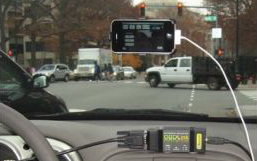
\includegraphics[width=0.7\textwidth]{SignalGuru}
    \caption[Signal Guru]{Signal Guru muss in der Lage sein die Ampel zu 'sehen'.  Quelle: \cite{SignalGuruPaper}} \label{fig:AppSignalGuru}
\end{figure}
\textit{Ob das auch in Deutschland funktioniert ist schwer zu sagen, da die Ampeln hierzulande so gesetzt sind, dass das Smartphone in der Pole-Position die Ampel evtl. nicht erfassen kann. Dies gilt es in der Entwicklungsarbeit zu testen und gegebenenfalls auszuarbeiten.}
%%% AMPELMETER %%%
\subsection{Ampelmeter}
\textbf{= Lorem Ipsum: gibt/gabs es die App wirklich? \\}
Ampelmeter ist eine Anwendung, die eine Geschwindigkeitsempfehlung angibt, bei der man die in Fahrtrichtung nächste Ampel bei grün erreichen. Der zweite Anwendungsfall ist die Restrot- bzw. Restgrünanzeige. Da der timingbezogene Teil der Datenbank zum Startzeitpunkt noch leer ist, bedarf es der Mitarbeit der NutzerInnen.
\section{Fahrraderweiterungen}
Als Schnittstelle das Smarthone nutzend gibt es ausgeklügelte Systeme mit reichlich Funktionen. Das einfache Navigationssystem für Fahrräder ist kaum noch notwendig, wo doch zum Beispiel die hier aufgeführten um einiges umfangreicher sind.
\subsection{Displaylose Fahrradnavigation}
Das \textsc{Hammerhead} ist ein "'Hammer"', oder einfach ein "'T"', an den Lenker angebracht und gespickt mit verschiedenfarbigen \gls{LED}s zeigt es den Weg zeigen, warnt vor Hindernissen und ersetzt die vorderen Scheinwerfer.
\begin{figure}[H]
    \centering
    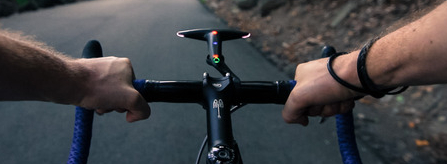
\includegraphics[width=0.7\textwidth]{hammerhead}
    \caption[Hammerhead]{LEDs zeigen den Weg.  Quelle: \url{http://blog.hammerhead.io/}} \label{fig:hammerhead}
\end{figure}
Via Bluetooth ist \textsc{Hammerhead} an das Smartphone gekoppelt, auf dem die zugehörige Navigationsanwendung läuft mit der man Routen eingeben, teilen und speichern kann\footnote{\cite{Hammerhead}}.\\
 Ein sehr ähnliches Prinzip verfolgt das \textsc{CycleNav} von der Firma Schwinn. Untersiede findet man hier im Design und integriertem Lautsprecher, der Abbiegehinweise ausgibt und auf Wunsch wiederholt\footnote{\cite{CycleNav}}.
\subsection{Intelligente Fahrradlenker}
Mehr High-Tech, aber auch umfangreichere Funktionen bietet der vom amerikanischen Startup \textsc{Helios-Bikes} entwickelte \textsc{Helios}-Lenker. Neben dem Frontlicht hat der Lenker wie in \ref{fig:helios} zu sehen, an den Enden \gls{LED}s die einen zum gewünschten Standort leiten. 
\begin{figure}[H]
    \centering
    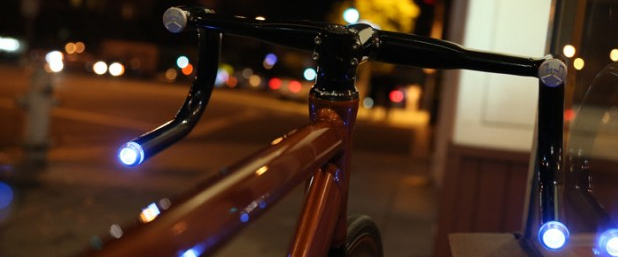
\includegraphics[width=0.7\textwidth]{helios}
    \caption[Helios-Lenker]{Helios-Lenker.  Quelle: \url{http://www.ridehelios.com/products.php}} \label{fig:helios}
\end{figure}
Sie passen ihre Farbe der Geschwindigkeit an und haben auf Wunsch auch eine Blinkfunktion. Verbindet man den Lenker mit einem Smartphone, lässt sich die Farbe der \gls{LED}s individualisieren. Die Verbindung zum Handy hat weitere Vorteile: dank des eingebauten \gls{GPS}-Trackers und eingesteckter SIM-Karte lässt sich das Fahrrad per SMS über den derzeitigen Standort abfragen\footnote{\cite{Helios}}, was im Falle eines Diebstahl sehr hilfreich sein kann.\\
\textsc{Vanhawks Valour} heißt das Rad, das ab April 2015 lieferbar ist. Wie im \textsc{Helios}-Lenker steckt auch hier ein über das Smartphon steuerbares Navigationssystem, das die Abbiegehinweise per \gls{LED} signalisiert, im Lenker. Auf den gefahrenen Routen merkt sich das Rad durch einen Erschütterungssensor erfasste Hindernisse wie Unebenheiten in der Fahrbahn und ermittelt beim nächsten Mal darauf rücksicht nehmend eine andere Route. Es ist darüber hinaus in der Lage mit anderen \textsc{Vanhawks valour}-Rädern zu kommunizieren und dessen Routenbegebenheiten ebenfalls zu berücksichtigen. Mittels Radarsensoren registriert das Fahrrad Autos im toten Winkel und benachrichtig die FahrerInnen durch ein vibrierenden Lenker\footnote{\cite{vanhawks}}.
%bluetooth kommunikation ... Akku im Rad wird mit Hilfe des Nabendynamos aufgeladen. yeah! App hat auch fitnesstrainer
\subsection{Das Samsung Smart Bike}
Auf der Mailänder Designwoche hat Samsung ein Smartbike vorgestellt, das mit verschiedenen intelligenten Komponenten wie Bluetooth, einer Kamera und Laserprojektoren ausgestattet. Der Rahmen ist aus Aluminium und leicht geschwungen, was Vibrationen abfangen soll. Wie \ref{fig:samsung} zeigt, zeichnen vier Laserprojektoren den eigenen, begleitenden Fahrradweg auf die Straße und sollen so die Sicherheit erhöhen, indem sie den Sicherheitsabstand markieren und aus dem toten Winkel sichtbar sind. 
\begin{figure}[H]
    \centering
    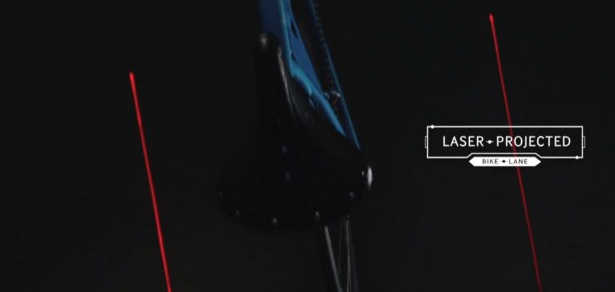
\includegraphics[width=0.7\textwidth]{samsung}
    \caption[Samsung Smart Bike]{Helios-Lenker.  Quelle: \url{http://www.maestrosacademy.it/progetto-sbike}} \label{fig:samsung}
\end{figure}
Natürlich ist auch dieses Fahrrad mit dem Smartphone verbunden, das sich dank eines Magneten einfach am Lenker anbringen lässt. Darüber kann man die Laserprojektoren ein- und ausschalten, dafür einen Timer bestimmen und über die eingebaute Kamera unter dem Sattel den Verkehr hinter sich im Auge behalten. Das Smartphone fungiert außerdem als Navigationsgerät und durch den eingebauten \gls{GPS}-Empfänger lassen eigene und Routen von anderen Nutzern speichern und intelligent verarbeiten\footnote{\cite{smartbike}}. Wenn also viele Menschen mit einem Samsung Smartbike unterwegs sind, erkennt das Rad die Route als angenehm und navigiert dort entlang. 
\subsection{Der COBI Fahrradcomputer}
Ein Kickstarterprojekt aus Frankfurt am Main entwickelt das System \textsc{COBI} (Connected Biking), das alle standardisierten Fahrradsysteme wie Lampen, Navigation, Tachometer etc. vereinen soll. \textsc{COBI} ist ein Modul mit inegrierter Frontleuchte in das man das Smartphone, welches dann mit der installierten \textsc{COBI}-App als Fahhradcomputer dient, legt. Durch eine wasser- und sto"ßfeste Hülle ist es vor Umwelteinflüssen geschützt. Zu dem Lenkersystem gibt es auch Rückstrahler beim Bremsen intensiver leuchten und eine Blinkfunktion haben.
\begin{figure}
        \centering
        \begin{subfigure}[b]{0.5\textwidth}
                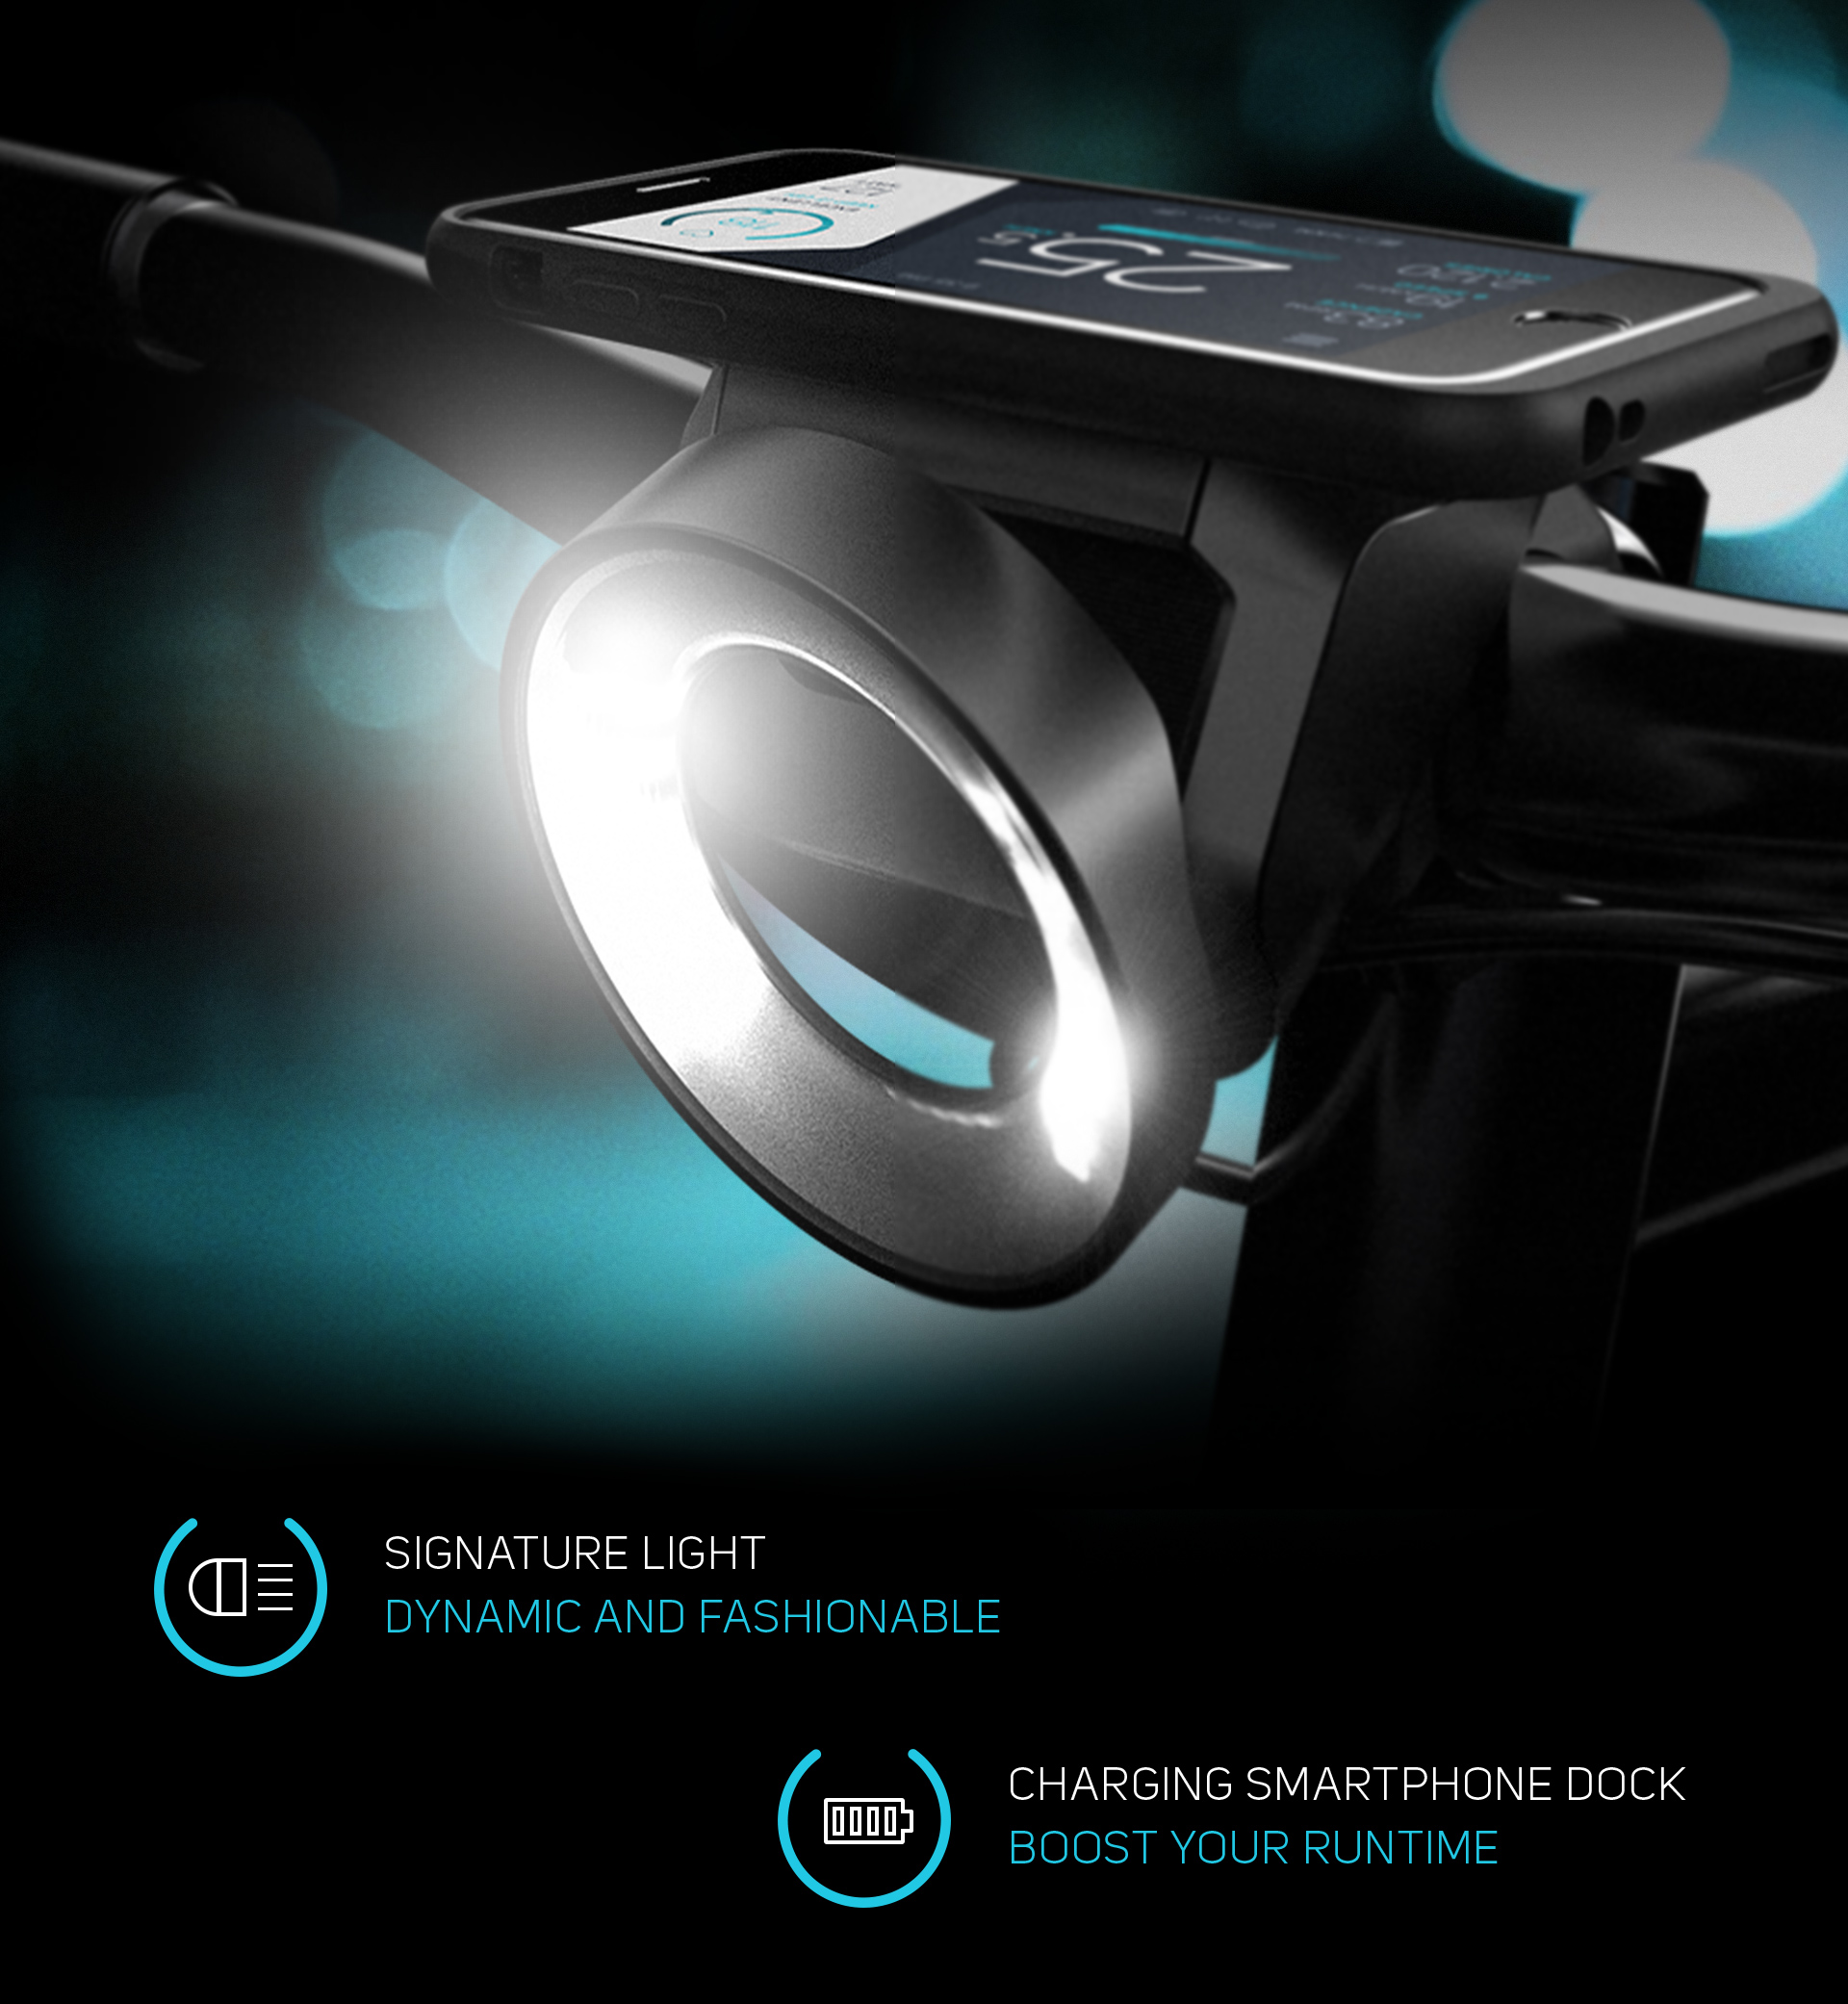
\includegraphics[width=\textwidth]{COBI_01}
                \caption{Frontlicht und Smartphonehalterung}
                \label{fig:cobi1}
        \end{subfigure}%
        ~ %add desired spacing between images, e. g. ~, \quad, \qquad, \hfill etc.
          %(or a blank line to force the subfigure onto a new line)
        \begin{subfigure}[b]{0.5\textwidth}
                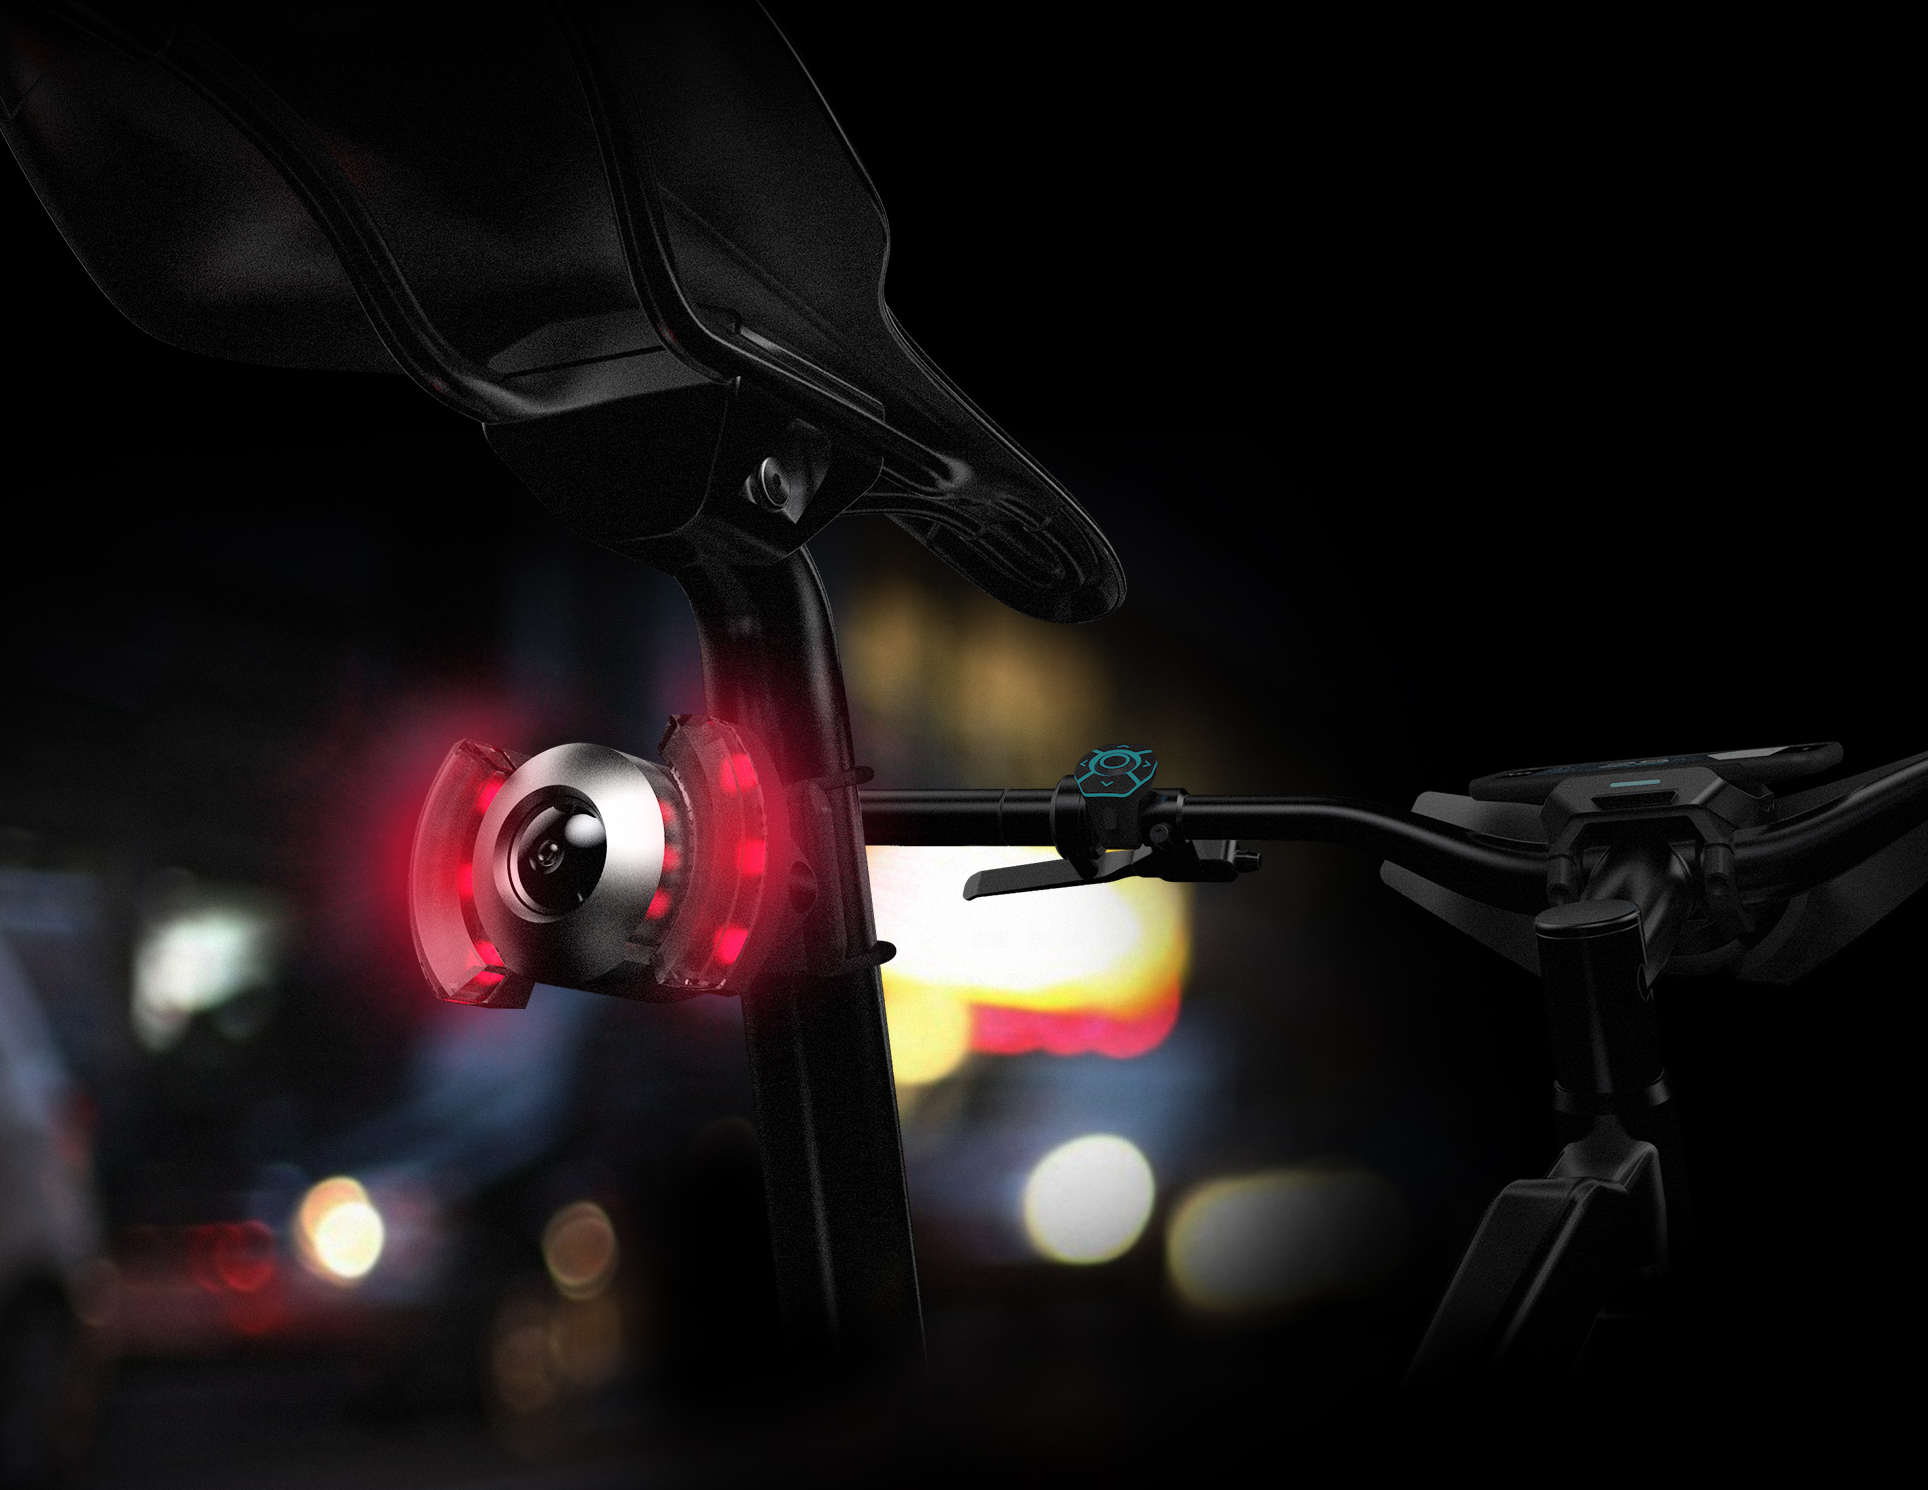
\includegraphics[width=\textwidth]{COBI_02}
                \caption{Bremslicht und Blinker}
                \label{fig:cobi}
        \end{subfigure}
        \caption{COBI -- Das smarte Fahrradsystem Quelle: \url{http://www.cobi.bike}}\label{fig:cobi}
\end{figure}
Möchte man das Smartphone trotzdem nicht am Lenker haben, bleibt die Verbindung zum Modul über Funk bestehen. Steuern lässt sich das System dann über einen Controller, den man am Lenker angebracht, mit dem Daumen bedienen kann. Ist es jedoch in der Halterung, wird das Smartphone über den E-Bike-Akku oder einen zusätzlich integrierten Akku aufgeladen. Wie bei den anderen genannten Systemen ist in der \textsc{COBI}-App eine Navigationsanwendung, wie auch die tracking&share Funktion inklusive. Darüber hinaus verfügt es über einen Diebstahlschutz, Fitnesstracker sowie die Möglichkeit einer Anbindung an Spotify\footnote{ Digitaler Musikstreaming Dienst}\footnote{\cite{cobi}}.\\
Das Projekt ist bereits voll finanziert und der Versand der vorbestellten Systeme beginnt vorrausichtlich im Frühjahr 2015.
%%% ERGIBNIS %%%
\section{Analyseergebnis}
Diese Beispiele zeigen deutlich, dass sowohl die Nachfrage nach Ampelassistenten -- mobil oder statisch -- als auch an Fahrraderweiterungen steigt und auf dem Markt Anklang findet. Auch die EntwicklerInnen solcher Systeme werden kreativer, wodurch immer mehr Produkte mit erweiterten Funktionen entstehen. Das begeistert wiederum mehr Menschen für das Radfahren und so ist der Verkehr flüssiger, die Teilnehmer entspannter, die Luft sauberer. AutofahrerInnen sind schon lange nicht mehr allein auf der Straße und so gilt es, dieses erfolgreiche Konzept für alle VerkehrsteilnehmerInnen zu erweitern.
